\documentclass{beamer}
\usepackage[utf8]{inputenc}
\usepackage{graphicx, epsfig}
\usepackage{amsmath,mathrsfs,amsfonts,amssymb}
\usepackage{floatflt}
\usepackage{epic,ecltree}
\usepackage{mathtext}
\usepackage{fancybox}
\usepackage{fancyhdr}
\usepackage{multirow}
\usepackage{enumerate}
\usepackage{epstopdf}
\usepackage{multicol}
\usepackage{algorithm}
\usepackage[noend]{algorithmic}
\usepackage{tikz}
\usepackage{blindtext}
\usetheme{default}%{Singapore}%{Warsaw}%{Warsaw}%{Darmstadt}
\usecolortheme{default}

\setbeamerfont{title}{size=\Huge}
\setbeamertemplate{footline}[page number]{}

\setbeamertemplate{section in toc}[sections numbered]


\makeatletter
\newcommand\HUGE{\@setfontsize\Huge{35}{40}}
\makeatother    

\setbeamerfont{title}{size=\HUGE}
\beamertemplatenavigationsymbolsempty

% latin bold lower
\newcommand{\ba}{\mathbf{a}} 
\newcommand{\bc}{\mathbf{c}} 
\newcommand{\be}{\mathbf{e}} 
\newcommand{\bff}{\mathbf{f}} % \bf - for bold type
\newcommand{\bg}{\mathbf{g}} 
\newcommand{\bh}{\mathbf{h}} 
\newcommand{\bp}{\mathbf{p}} 
\newcommand{\bq}{\mathbf{q}} 
\newcommand{\bt}{\mathbf{t}} 
\newcommand{\bs}{\mathbf{s}} 
\newcommand{\bu}{\mathbf{u}} 
\newcommand{\bv}{\mathbf{v}} 
\newcommand{\bw}{\mathbf{w}} 
\newcommand{\bx}{\mathbf{x}} 
\newcommand{\by}{\mathbf{y}} 
\newcommand{\bz}{\mathbf{z}} 

% latin bold upper
\newcommand{\bA}{\mathbf{A}} 
\newcommand{\bB}{\mathbf{B}} 
\newcommand{\bC}{\mathbf{C}} 
\newcommand{\bG}{\mathbf{G}} 
\newcommand{\bI}{\mathbf{I}} 
\newcommand{\bJ}{\mathbf{J}} 
\newcommand{\bL}{\mathbf{L}} 
\newcommand{\bM}{\mathbf{M}} 
\newcommand{\bP}{\mathbf{P}}
\newcommand{\bQ}{\mathbf{Q}} 
\newcommand{\bR}{\mathbf{R}} 
\newcommand{\bT}{\mathbf{T}} 
\newcommand{\bU}{\mathbf{U}} 
\newcommand{\bV}{\mathbf{V}} 
\newcommand{\bW}{\mathbf{W}} 
\newcommand{\bX}{\mathbf{X}} 
\newcommand{\bY}{\mathbf{Y}} 
\newcommand{\bZ}{\mathbf{Z}} 

% latin cal upper
\newcommand{\cF}{\mathcal{F}} 
\newcommand{\cG}{\mathcal{G}} 
\newcommand{\cI}{\mathcal{I}} 
\newcommand{\cL}{\mathcal{L}} 
\newcommand{\cM}{\mathcal{M}} 
\newcommand{\cN}{\mathcal{N}} 
\newcommand{\cP}{\mathcal{P}} 
\newcommand{\cS}{\mathcal{S}} 
\newcommand{\cT}{\mathcal{T}} 
\newcommand{\cW}{\mathcal{W}} 
\newcommand{\cX}{\mathcal{X}} 
\newcommand{\cZ}{\mathcal{Z}} 

% latin bb upper
\newcommand{\bbE}{\mathbb{E}} 
\newcommand{\bbI}{\mathbb{I}} 
\newcommand{\bbP}{\mathbb{P}} 
\newcommand{\bbR}{\mathbb{R}} 

% greek bold lower
\newcommand{\bepsilon}{\boldsymbol{\epsilon}} 
\newcommand{\btheta}{\boldsymbol{\theta}} 
\newcommand{\blambda}{\boldsymbol{\lambda}} 
\newcommand{\bpi}{\boldsymbol{\pi}} 
\newcommand{\bmu}{\boldsymbol{\mu}} 
\newcommand{\bsigma}{\boldsymbol{\sigma}} 
\newcommand{\bphi}{\boldsymbol{\phi}} 

% greek bold upper
\newcommand{\bSigma}{\boldsymbol{\Sigma}} 

\DeclareMathOperator*{\argmin}{arg\,min}
\DeclareMathOperator*{\argmax}{arg\,max}

\newcommand{\createdgmtitle}[1]{\title[\hbox to 56mm{Deep Generative Models  \hfill\insertframenumber\,/\,\inserttotalframenumber}]
	{\vspace{1cm} \\ \textbf{Deep Generative Models} \\ {\Huge Lecture #1}}
	\author{Roman Isachenko}
		\institute{
\includegraphics[width=0.7cm]{../utils/aimasterslogo} \LARGE{AI Masters}}
	\date{2024, Summer}
}

\usepackage{tikz}
\usetikzlibrary{arrows,shapes,positioning,shadows,trees}

\newcommand\myfootnote[1]{%
  \tikz[remember picture,overlay]
  \draw (current page.south west) +(1in + \oddsidemargin,0.5em)
  node[anchor=south west,inner sep=0pt]{\parbox{\textwidth}{%
      \rlap{\rule{10em}{0.4pt}}\raggedright\scriptsize \textit{#1}}};}

\newcommand\myfootnotewithlink[2]{%
  \tikz[remember picture,overlay]
  \draw (current page.south west) +(1in + \oddsidemargin,0.5em)
  node[anchor=south west,inner sep=0pt]{\parbox{\textwidth}{%
      \rlap{\rule{10em}{0.4pt}}\raggedright\scriptsize\href{#1}{\textit{#2}}}};}
      
\AtBeginSection[]
      {
      	\begin{frame}{Outline}
      		\tableofcontents[currentsection]
      	\end{frame}
      }
      \AtBeginSubsection[]{
      	\begin{frame}{Outline}
      		\tableofcontents[currentsection,currentsubsection]
      	\end{frame}
}
\createdgmtitle{2}

\usepackage{tikz}

\usetikzlibrary{arrows,shapes,positioning,shadows,trees}
%--------------------------------------------------------------------------------
\begin{document}
%--------------------------------------------------------------------------------
\begin{frame}[noframenumbering,plain]
%\thispagestyle{empty}
\titlepage
\end{frame}
%======
\begin{frame}{Recap of previous lecture}
	We are given i.i.d. samples $\{\bx_i\}_{i=1}^n \in \bbR^m$ from unknown distribution $\pi(\bx)$.

	\begin{block}{Goal}
		We would like to learn a distribution $\pi(\bx)$ for 
		\begin{itemize}
		    \item evaluating $\pi(\bx)$ for new samples (how likely to get object $\bx$?);
		    \item sampling from $\pi(\bx)$ (to get new objects $\bx \sim \pi(\bx)$).
		\end{itemize}
	\end{block}
	Instead of searching true $\pi(\bx)$ over all probability distributions, learn function approximation $p(\bx | \btheta) \approx \pi(\bx)$.
	\begin{block}{Divergence}
		\begin{itemize}
			\item $D(\pi || p) \geq 0$ for all $\pi, p \in \cP$;
			\item $D(\pi || p) = 0$ if and only if $\pi \equiv p$.
		\end{itemize}
	\end{block}
	\begin{block}{Divergence minimization task}
		\vspace{-0.3cm}
		\[
		\min_{\btheta} D(\pi || p).
		\]
	\end{block}
\end{frame}
%=======
\begin{frame}{Recap of previous lecture}
	\begin{block}{Forward KL}
		\vspace{-0.2cm}
		\[
		KL(\pi || p) = \int \pi (\bx) \log \frac{\pi(\bx)}{p(\bx | \btheta)} d \bx \rightarrow \min_{\btheta}
		\]
	\end{block}
	\begin{block}{Reverse KL}
		\vspace{-0.2cm}
		\[
		KL(p || \pi) = \int p (\bx| \btheta) \log \frac{p(\bx| \btheta)}{\pi(\bx)} d \bx \rightarrow \min_{\btheta}
		\]
	\end{block}
	
	\begin{block}{Maximum likelihood estimation (MLE)}
		\vspace{-0.3cm}
		\[
		\btheta^* = \argmax_{\btheta} \prod_{i=1}^n p(\bx_i | \btheta) = \argmax_{\btheta} \sum_{i=1}^n \log p(\bx_i | \btheta).
		\]
		\vspace{-0.1cm}
	\end{block}
	Maximum likelihood estimation is equivalent to minimization of the Monte-Carlo estimate of forward KL.
\end{frame}
%=======
\begin{frame}{Recap of previous lecture}
	\begin{block}{Likelihood as product of conditionals}
		Let $\bx = (x_1, \dots, x_m)$, $\bx_{1:j} = (x_1, \dots, x_j)$. Then 
		\[
		p(\bx | \btheta) = \prod_{j=1}^m p(x_j | \bx_{1:j - 1}, \btheta); \quad 
		\log p(\bx | \btheta) = \sum_{j=1}^m \log p(x_j | \bx_{1:j - 1}, \btheta).
		\]
	\end{block}
	\vspace{-0.3cm}
	\begin{block}{MLE problem for autoregressive model}
		\vspace{-0.3cm}
		\[
		\btheta^* = \argmax_{\btheta} \sum_{i=1}^n \sum_{j=1}^m \log p(x_{ij} | \bx_{i, 1:j - 1}\btheta).
		\]
		\vspace{-0.5cm}
	\end{block}
	\begin{block}{Sampling}
		\vspace{-0.5cm}
		\[
		{\color{teal}\hat{x}_1} \sim p(x_1 | \btheta), \quad \hat{x}_2 \sim p(x_2 | {\color{teal}\hat{x}_1}, \btheta), \quad \dots, \quad \hat{x}_m \sim p(x_m | \hat{\bx}_{1:m-1}, \btheta)
		\]
		New generated object is $\hat{\bx} = (\hat{x}_1, \hat{x}_2, \dots, \hat{x}_m)$.
	\end{block}
\end{frame}
%=======
\begin{frame}{Outline}
	\tableofcontents
\end{frame}
%=======
\section{Autoregressive models (continued)}
%=======
\begin{frame}{Autoregressive models: MLP}
	For large $j$ the conditional distribution $p(x_j | \bx_{1:j - 1}, \btheta)$ could be infeasible. Moreover, the history $\bx_{1:j-1}$ has non-fixed length.
	\begin{block}{Markov assumption}
		\vspace{-0.5cm}
		\[
			p(x_j | \bx_{1:j - 1}, \btheta) = p(x_j | \bx_{j - d:j - 1}, \btheta), \quad d \text{ is a fixed model parameter}.
		\]
	\end{block}
	\vspace{-0.5cm}
	\begin{block}{Example}
		\begin{minipage}[t]{0.39\columnwidth}
			{\small
			\begin{itemize}
				\item $d = 2$;
				\item $x_j \in \{0, 255\}$;
				\item $\bh_j = \text{MLP}_{\btheta}(x_{j - 1}, x_{j - 2})$;
				\item $\bpi_j = \text{softmax}(\bh_j)$;
				\item $p(x_j | x_{j - 1}, x_{j - 2}, \btheta) = \text{Categorical}(\bpi_j)$.
			\end{itemize}
			}
		\end{minipage}%
		\begin{minipage}[t]{0.61\columnwidth}
			 \begin{figure}
			   \centering
			   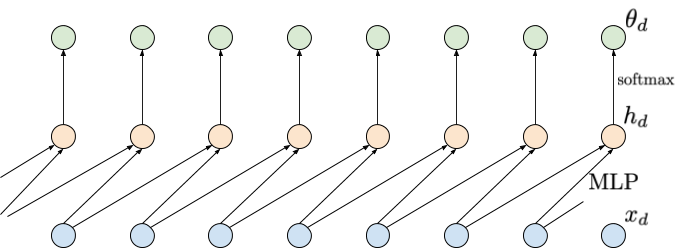
\includegraphics[width=1.0\linewidth]{figs/sequential_MLP}
			 \end{figure}
			 Is it possible to model continuous distributions instead of discrete one?
		\end{minipage}
	\end{block}
	 \myfootnotewithlink{https://jmtomczak.github.io/blog/2/2\_ARM.html}{image credit: https://jmtomczak.github.io/blog/2/2\_ARM.html}
\end{frame}
%=======
\begin{frame}{Autoregressive models: PixelCNN}
	\begin{block}{Goal}
		Model a distribution $\pi(\bx)$ of natural images.
	\end{block}
	\begin{block}{Solution}
		Autoregressive model on 2D pixels
		\[
		    p(\bx | \btheta) = \prod_{j=1}^{\text{width} \times \text{height}} p(x_j|\bx_{1:j-1}, \btheta).
		\]
		\begin{itemize}
			\item We need to introduce the ordering of image pixels.
		    \item The convolution should be \textbf{masked} to make them causal.
		    \item The image has RGB channels, these dependencies could be addressed.
		\end{itemize}
	\end{block}
	\myfootnotewithlink{https://arxiv.org/abs/1601.06759}{Oord A., Kalchbrenner N., Kavukcuoglu K. Pixel recurrent neural networks, 2016}
\end{frame}
%=======
\begin{frame}{Autoregressive models: PixelCNN}
	\vspace{-0.2cm}
	\begin{minipage}[t]{0.5\columnwidth}
		\begin{block}{Raster ordering}
			\begin{figure}
				\centering
		        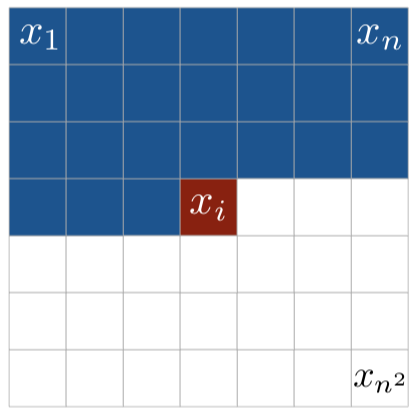
\includegraphics[width=0.7\linewidth]{figs/pixelcnn1.png}
			\end{figure}
		\end{block}
		\vspace{-0.5cm}
		\begin{block}{Mask for the convolution kernel}
			\begin{figure}
				\centering
		        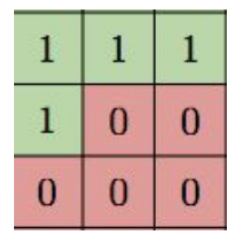
\includegraphics[width=0.35\linewidth]{figs/pixelcnn_0_1.png}
			\end{figure}
		\end{block}
	\end{minipage}%
	\begin{minipage}[t]{0.5\columnwidth}
		\begin{block}{Dependencies between pixels}
			\begin{figure}
				\centering
		        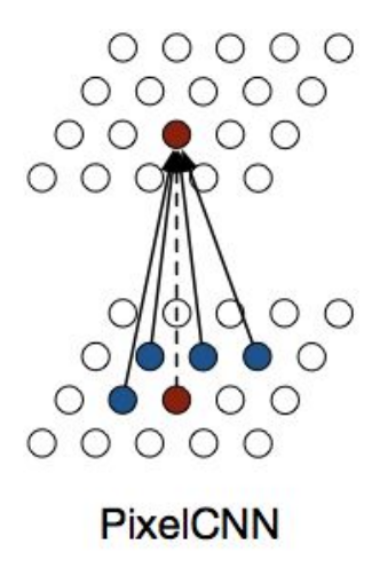
\includegraphics[width=0.5\linewidth]{figs/pixelcnn_0_2.png}
			\end{figure}
			\vspace{-0.3cm}
			\begin{figure}
				\centering
		        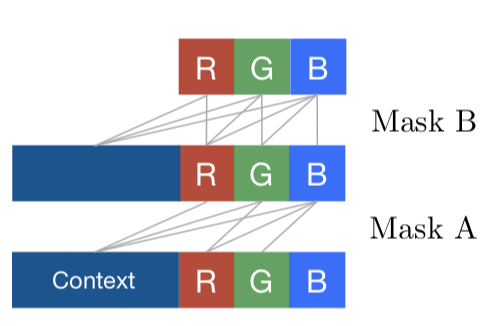
\includegraphics[width=0.65\linewidth]{figs/pixelcnn2.png}
			\end{figure}
		\end{block}
	\end{minipage}
	\myfootnotewithlink{https://arxiv.org/abs/1601.06759}{Oord A., Kalchbrenner N., Kavukcuoglu K. Pixel recurrent neural networks, 2016}
\end{frame}
%=======
\section{Normalizing flows (NF)}
%=======
\begin{frame}{Generative models zoo}
	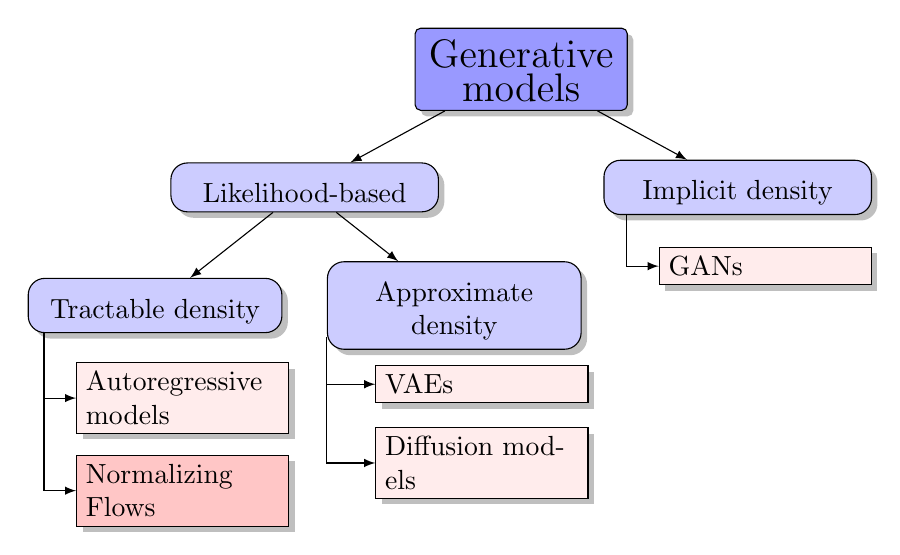
\begin{tikzpicture}[
	 	basic/.style  = {draw, text width=2cm, drop shadow, rectangle},
	 	root/.style   = {basic, rounded corners=2pt, thin, text height=1.1em, text width=7em, align=center, fill=blue!40},
	 	level 1/.style={sibling distance=55mm},
	 	level 2/.style = {basic, rounded corners=6pt, thin, align=center, fill=blue!20, text height=1.1em, text width=9em, sibling distance=38mm},
	 	level 3/.style = {basic, rounded corners=6pt, thin,align=center, fill=blue!20, text width=8.5em},
	 	level 4/.style = {basic, thin, align=left, fill=pink!30, text width=7em},
	 	level 5/.style = {basic, thin, align=left, fill=pink!90, text width=7em},
		edge from parent/.style={->,draw},
		>=latex]
		
		% root of the the initial tree, level 1
		\node[root] {\Large Generative models}
		% The first level, as children of the initial tree
		child {node[level 2] (c1) {Likelihood-based}
			child {node[level 3] (c11) {Tractable density}}
			child {node[level 3] (c12) {Approximate density}}
		}
		child {node[level 2] (c2) {Implicit density}};
		
		% The second level, relatively positioned nodes
		\begin{scope}[every node/.style={level 4}]
		\node [below of = c11, yshift=-5pt, xshift=10pt] (c111) {Autoregressive models};
		
		\node [below of = c12, xshift=10pt] (c121) {VAEs};
		\node [below of = c121] (c122) {Diffusion models};
		\node [below of = c2, xshift=10pt] (c21) {GANs};
		
		\end{scope}
		
		% The second level, relatively positioned nodes
		\begin{scope}[every node/.style={level 5}]
			\node [below of = c111, yshift=-5pt] (c112) {Normalizing Flows};
		\end{scope}
		
		
		% lines from each level 1 node to every one of its "children"
		\foreach \value in {1,2}
		\draw[->] (c11.194) |- (c11\value.west);
		
		\foreach \value in {1,2}
		\draw[->] (c12.194) |- (c12\value.west);
		
		\draw[->] (c2.194) |- (c21.west);
		
	\end{tikzpicture}
\end{frame}
%=======
\begin{frame}{Normalizing flows prerequisites}
	\begin{block}{Jacobian matrix}
		Let $\bff: \mathbb{R}^m \rightarrow \mathbb{R}^m$ be a differentiable function.
		\[
			\bz = \bff(\bx), \quad 
			\bJ =  \frac{\partial \bz}{\partial \bx} =
			\begin{pmatrix}
				\frac{\partial z_1}{\partial x_1} & \dots & \frac{\partial z_1}{\partial x_m} \\
				\dots & \dots & \dots \\ 
				\frac{\partial z_m}{\partial x_1} & \dots & \frac{\partial z_m}{\partial x_m}
			\end{pmatrix} \in \bbR^{m \times m}
		\]
		\vspace{-0.3cm}
	\end{block}
	\begin{block}{Change of variable theorem (CoV)}
		Let $\bx$ be a random variable with density function $p(\bx)$ and $\bff: \mathbb{R}^m \rightarrow \mathbb{R}^m$ is a differentiable, \textbf{invertible} function. If $\bz = \bff(\bx)$, $\bx = \bff^{-1}(\bz) = \bg(\bz)$, then
		\begin{align*}
			p(\bx) &= p(\bz) |\det(\bJ_{\bff})| = p(\bz) \left|\det \left( \frac{\partial \bz}{\partial \bx} \right) \right| = p(\bff(\bx)) \left|\det \left(  \frac{\partial \bff(\bx)}{\partial \bx} \right) \right| \\
			p(\bz) &= p(\bx) |\det(\bJ_{\bg})|= p(\bx) \left|\det \left(  \frac{\partial \bx}{\partial \bz} \right) \right| = p(\bg(\bz)) \left|\det \left(  \frac{\partial \bg(\bz)}{\partial \bz} \right) \right|.
		\end{align*}
		\vspace{-0.5cm}
	\end{block}
\end{frame}
%=======
\begin{frame}{Jacobian determinant}
	\begin{block}{Inverse function theorem}
		If function $\bff$ is invertible and Jacobian matrix is continuous and non-singular, then
		\vspace{-0.3cm}
		\[
		\bJ_{\bff^{-1}} = \bJ_{\bg} = \bJ_\bff^{-1}; \quad |\det (\bJ_{\bff^{-1}})| = |\det (\bJ_\bg)| = \frac{1}{|\det (\bJ_\bff)|}.
		\]
		\vspace{-0.3cm}
	\end{block}
	\begin{minipage}{0.55\columnwidth}
		\begin{itemize}
			\item $\bx$ and $\bz$ have the same dimensionality ($\bbR^m$).
			\vfill
			\item $\bff_{\btheta}(\bx)$ could be parametric function.
			\vfill
			\item Determinant  of Jacobian matrix $\mathbf{J} =\frac{\partial \bff_{\btheta}(\bx)}{\partial \bx}$ shows how the volume changes under the transformation.
		\end{itemize}
	\end{minipage}%
	\begin{minipage}{0.45\columnwidth}
		\begin{figure}
			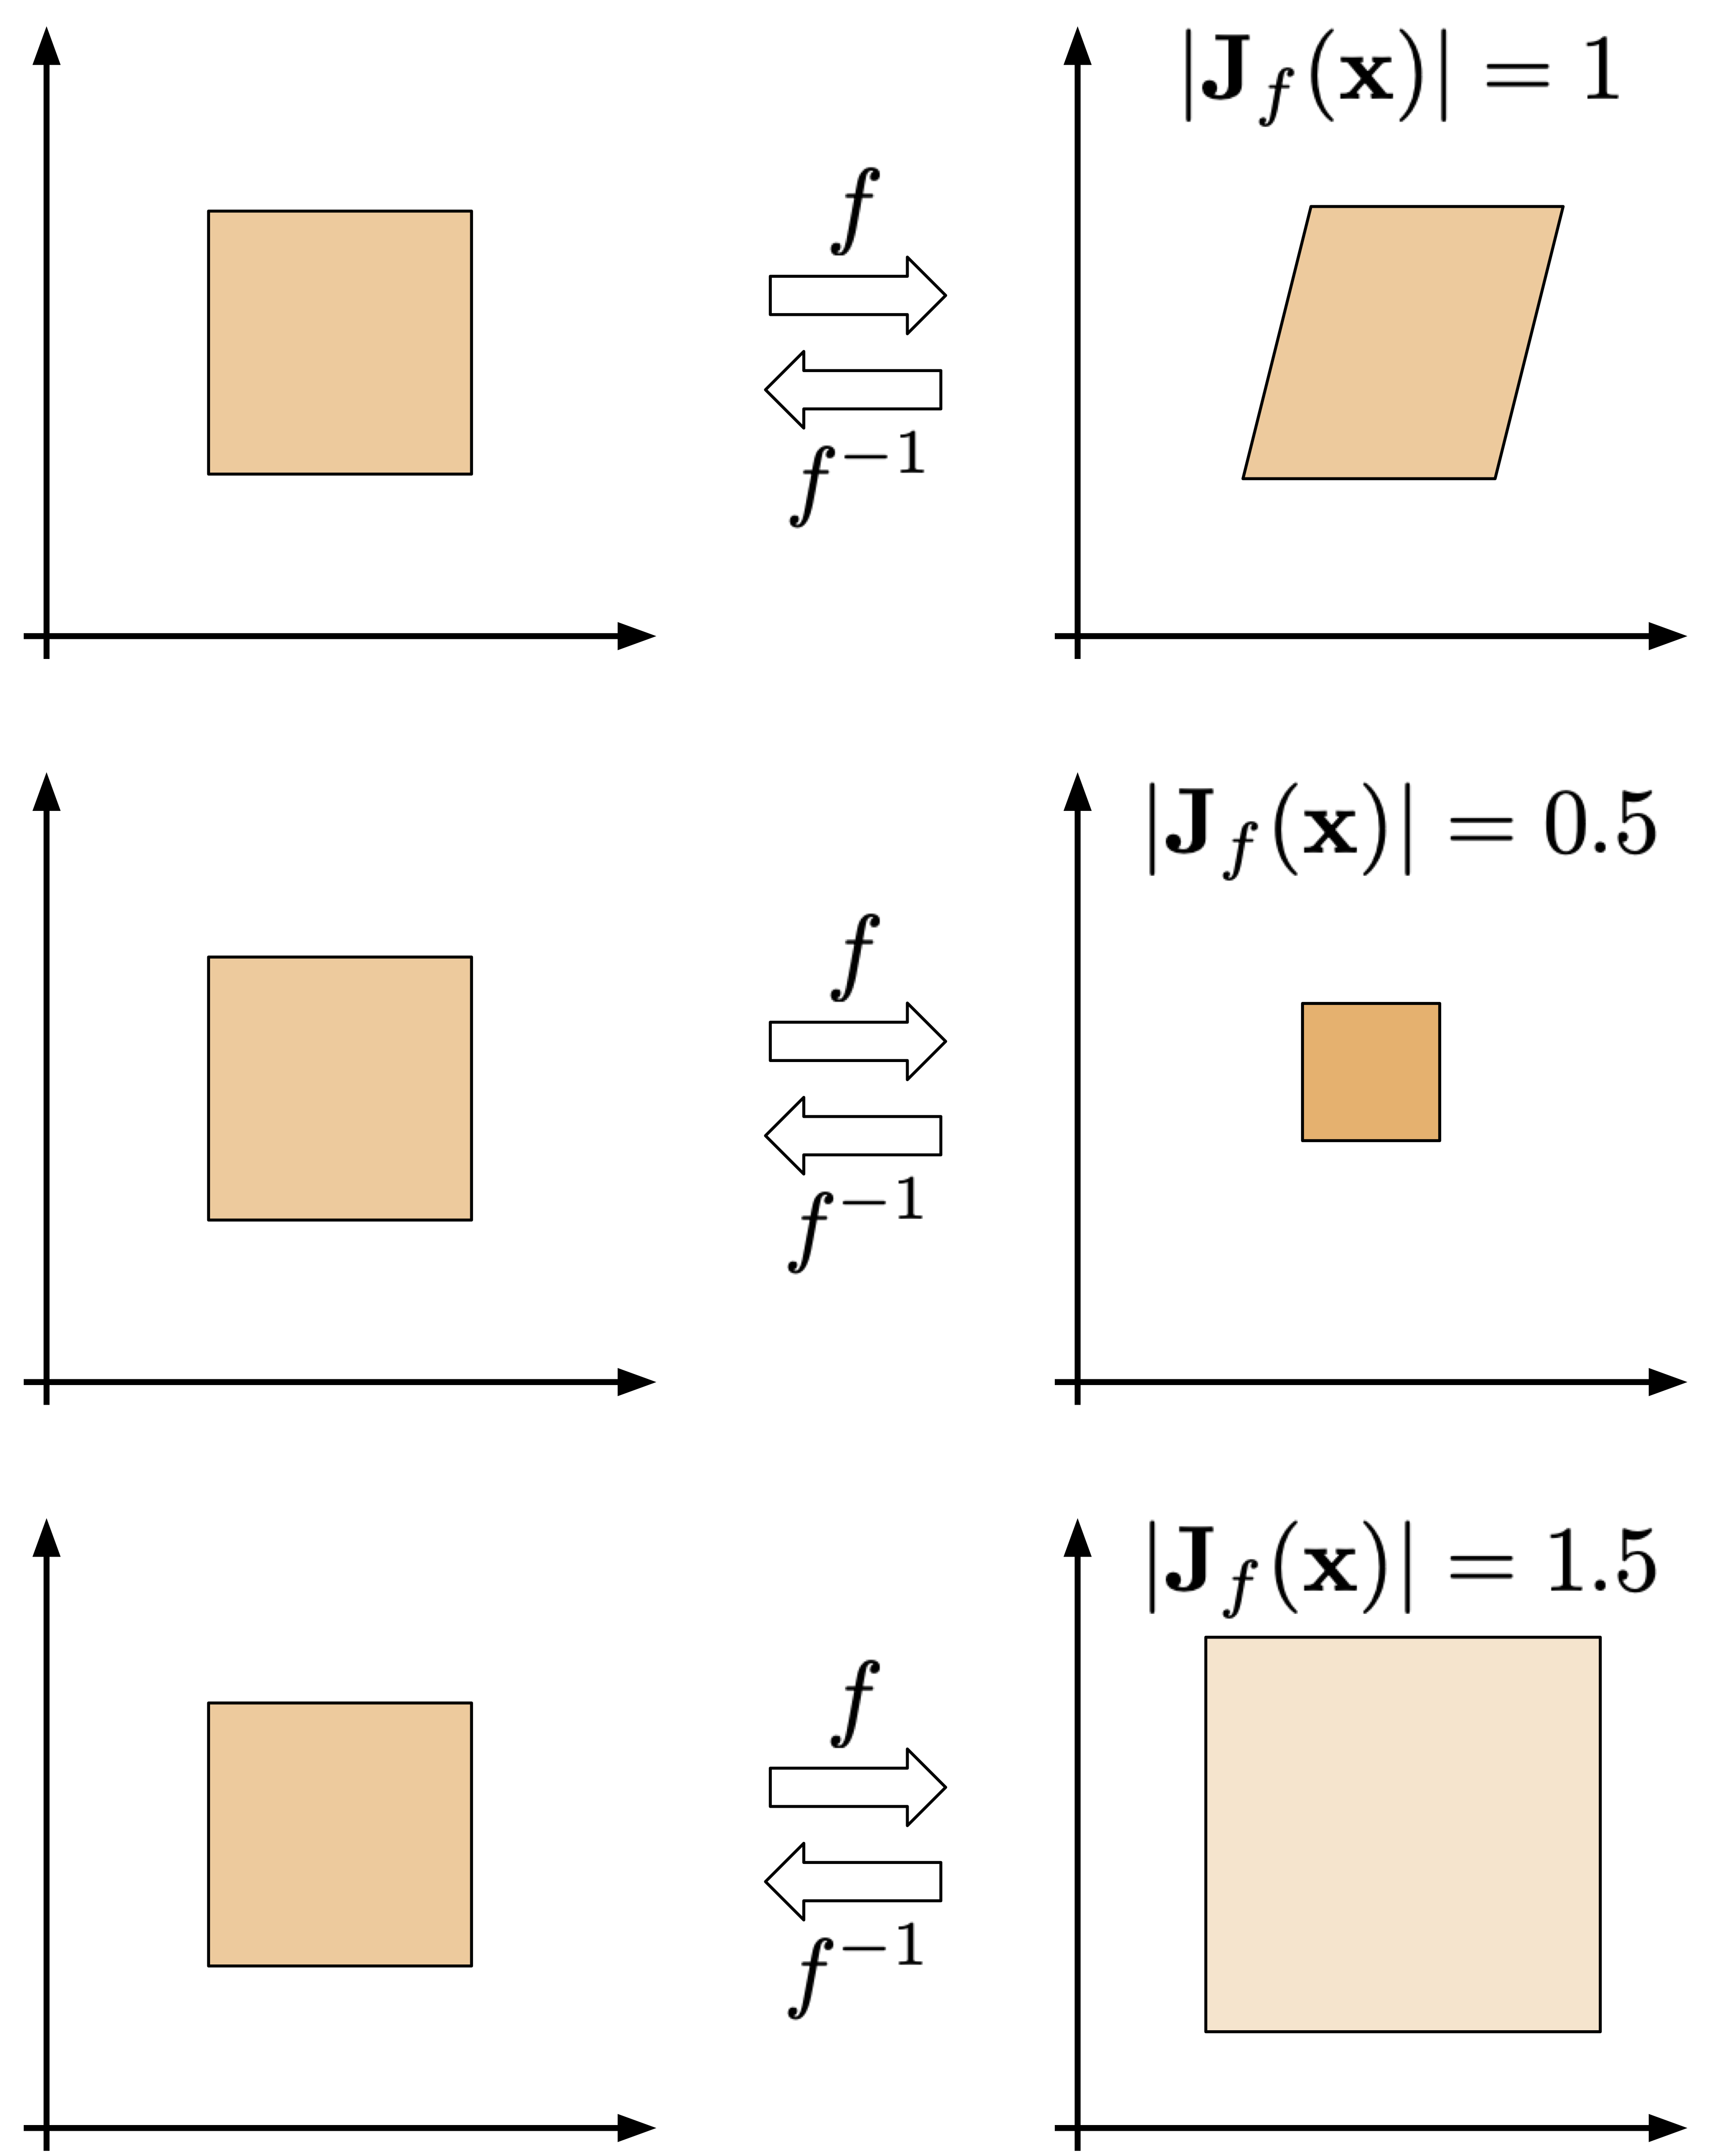
\includegraphics[width=0.8\linewidth]{figs/jacobian_det}
		\end{figure}
	\end{minipage}
	\myfootnotewithlink{https://jmtomczak.github.io/blog/3/3\_flows.html}{https://jmtomczak.github.io/blog/3/3\_flows.html}
\end{frame}
%=======
\begin{frame}{Fitting normalizing flows}
	\begin{block}{MLE problem}
		\vspace{-0.3cm}
		\[
		p(\bx|\btheta) = p(\bz) \left|\det \left(  \frac{\partial \bz}{\partial \bx} \right) \right|  = p(\bff_{\btheta}(\bx)) \left|\det \left( \frac{\partial \bff_{\btheta}(\bx)}{\partial \bx} \right) \right|
		\]
		\[
		\log p(\bx|\btheta) = \log p(\bff_{\btheta}(\bx)) + \log  |\det (\bJ_{\bff}) | \rightarrow \max_{\btheta}
		\]
	\end{block}
	\vspace{-0.2cm}
	\begin{figure}
		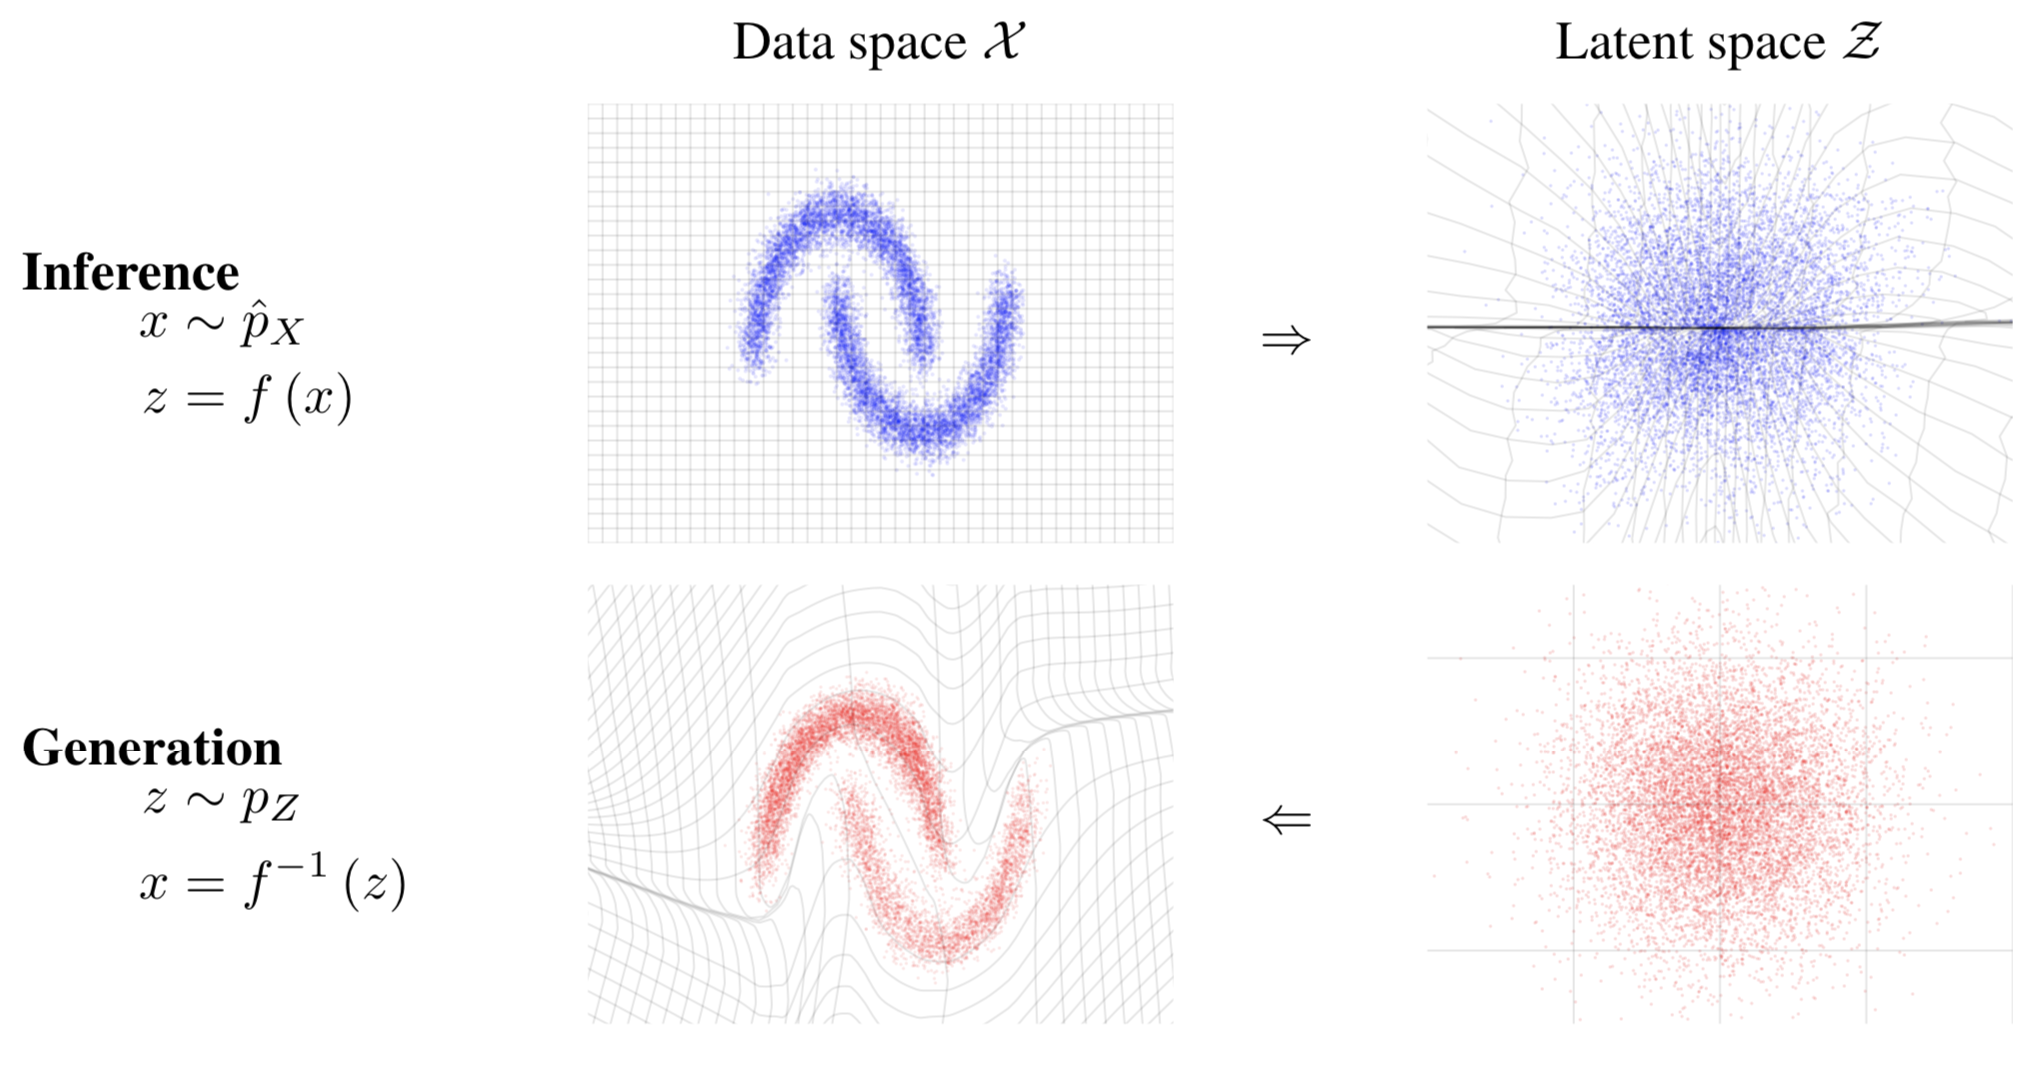
\includegraphics[width=0.85\linewidth]{figs/flows_how2}
	\end{figure}
	\myfootnotewithlink{https://arxiv.org/abs/1605.08803}{Dinh L., Sohl-Dickstein J., Bengio S. Density estimation using Real NVP, 2016} 
\end{frame}
%=======
\begin{frame}{Composition of normalizing flows}
	\begin{block}{Theorem}
		If $\{\bff_k\}_{k=1}^K$ satisfy conditions of the change of variable theorem, then $\bz = \bff(\bx) = \bff_K \circ \dots \circ \bff_1(\bx)$ also satisfies it.
	\end{block}
	\vspace{-0.5cm}
	{ \footnotesize
		\begin{multline*}
			p(\bx) = p(\bff(\bx)) \left|\det \left(\frac{\partial \bff(\bx)}{\partial \bx} \right) \right| =
			p(\bff(\bx)) \left|\det \left(\frac{\partial \textbf{f}_K}{\partial \textbf{f}_{K-1}} \dots \frac{\partial \textbf{f}_1}{\partial \bx} \right) \right| = \\ = p(\bff(\bx)) \prod_{k=1}^K \left|\det \left(\frac{\partial \textbf{f}_{k}}{\partial \textbf{f}_{k-1}} \right) \right|
			= p(\bff(\bx)) \prod_{k=1}^K |\det ( \bJ_{f_k}) |
		\end{multline*}
	}
	\vspace{-0.3cm}
	\begin{figure}
		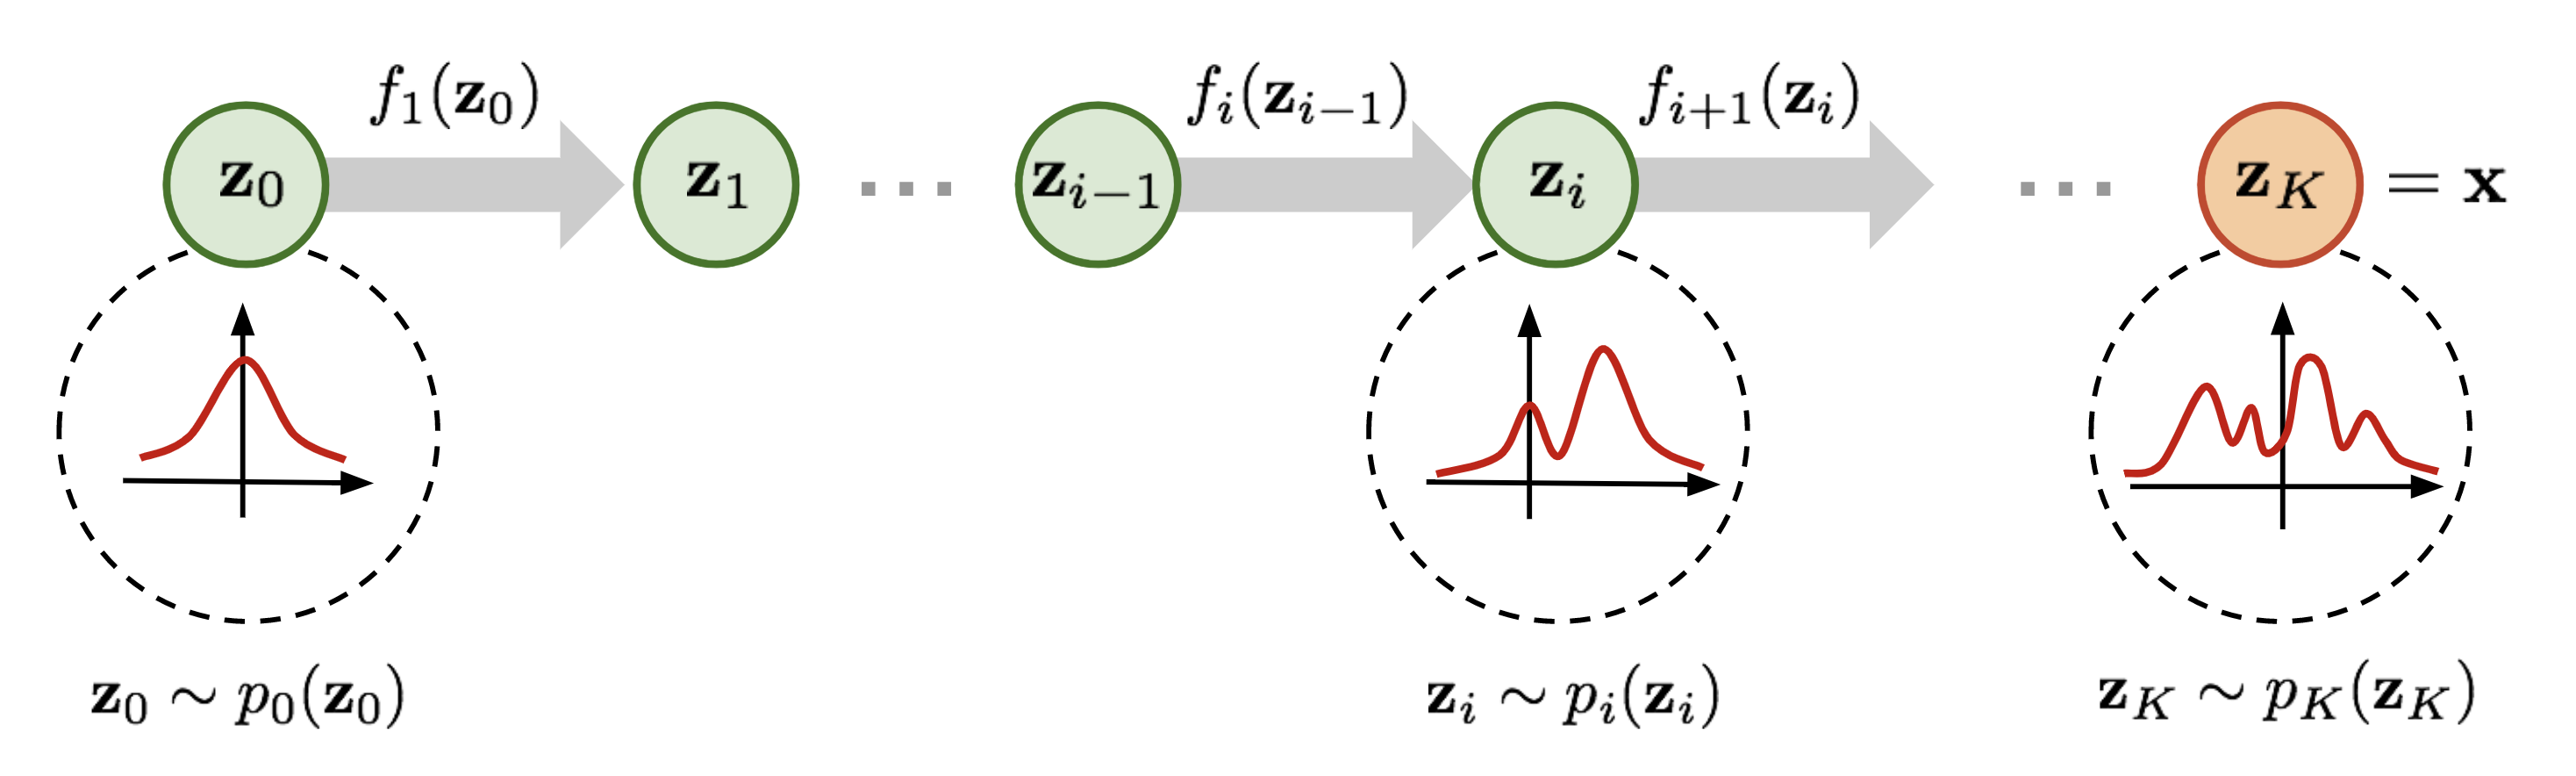
\includegraphics[width=0.95\linewidth]{figs/normalizing-flow}
	\end{figure}
	\myfootnotewithlink{https://lilianweng.github.io/lil-log/2018/10/13/flow-based-deep-generative-models.html}{https://lilianweng.github.io/lil-log/2018/10/13/flow-based-deep-generative-models.html}
\end{frame}
%=======
\begin{frame}{Normalizing flows (NF)}
	\vspace{-0.3cm}
	\[
	\log p(\bx|\btheta) = \log p(\bff_{\btheta}(\bx)) + \log |\det (\bJ_\bff)|
	\]
	\vspace{-0.4cm}
	\begin{block}{Definition}
		Normalizing flow is a \textit{differentiable, invertible} mapping from data $\bx$ to the noise $\bz$. 
	\end{block}
	\begin{itemize}
		\item \textbf{Normalizing} means that NF takes samples from $\pi(\bx)$ and normalizes them into samples from the density $p(\bz)$.
		\item \textbf{Flow} refers to the trajectory followed by samples from $p(\bz)$ as they are transformed by the sequence of transformations
		\[
		\bz = \bff_K \circ \dots \circ \bff_1(\bx); \quad \bx = \bff_1^{-1} \circ \dots \circ \bff_K^{-1} (\bz) = \bg_1 \circ \dots \circ \bg_K(\bz) 
		\] 
		\vspace{-0.4cm}
		\begin{block}{Log likelihood}
			\vspace{-0.4cm}
			\[
			\log p(\bx | \btheta) = \log p(\bff_K \circ \dots \circ \bff_1(\bx)) + \sum_{k=1}^K\log |\det (\bJ_{\bff_k})|,
			\]
			\vspace{-0.4cm} \\
			where $\bJ_{\bff_k} = \frac{\partial \mathbf{f}_k}{\partial \bff_{k-1}}$.
		\end{block}
	\end{itemize}
	\textbf{Note:} Here we consider only \textbf{continuous} random variables.
\end{frame}
%=======
\begin{frame}{Normalizing flows}
	\begin{block}{Example of a 4-step NF}
		\vspace{-0.2cm}
		\begin{figure}
			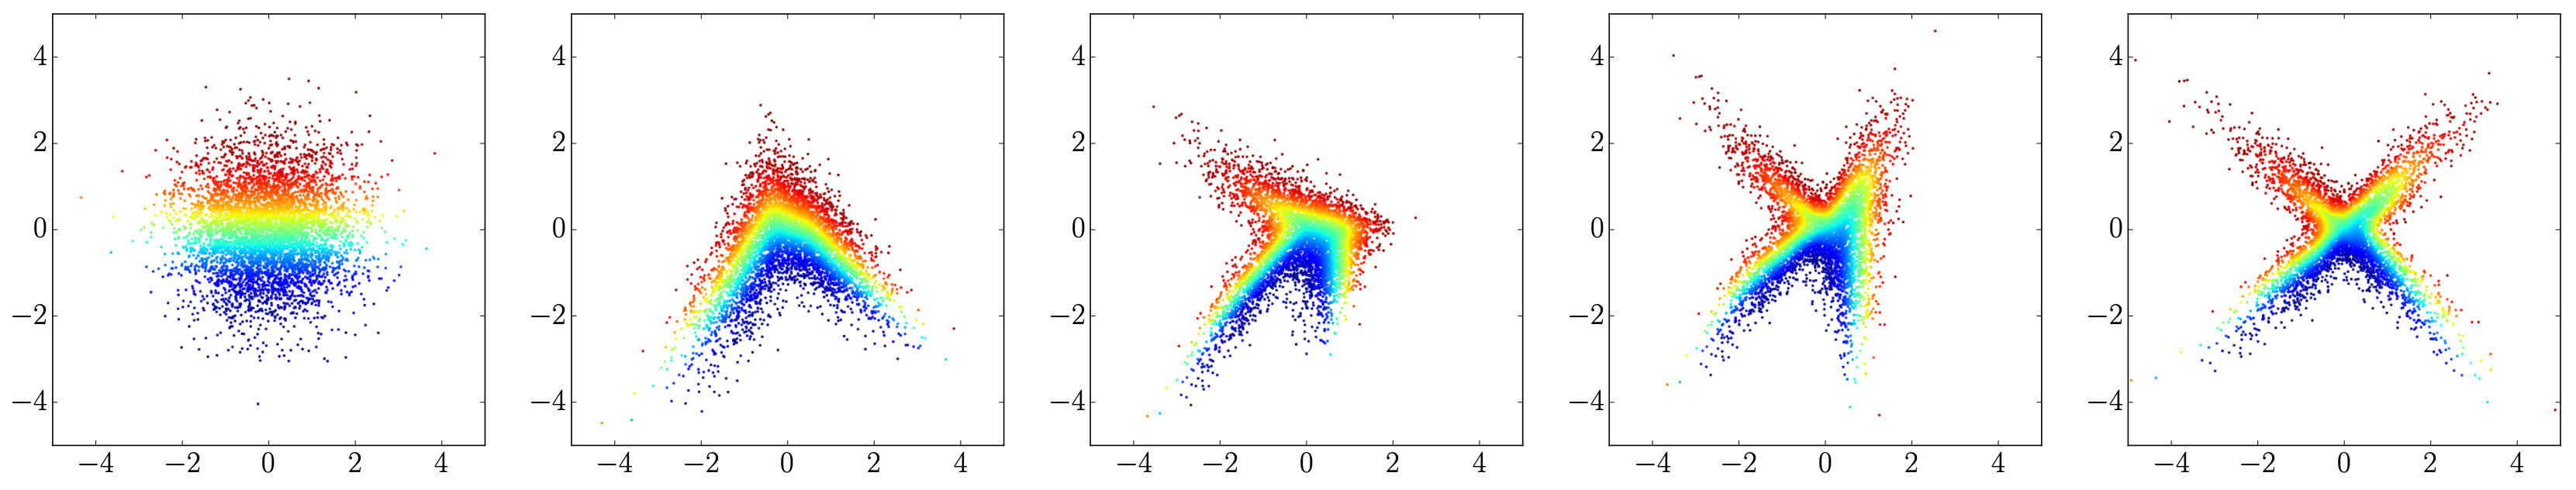
\includegraphics[width=\linewidth]{figs/flow_4_steps_example.png}
		\end{figure}
	\end{block}
	\vspace{-0.5cm}
	\begin{block}{NF log likelihood}
		\vspace{-0.3cm}
		\[
		\log p(\bx|\btheta) = \log p(\bff_{\btheta}(\bx)) + \log |\det ( \bJ_\bff)|
		\]
		\vspace{-0.3cm}
	\end{block}
	What is the complexity of the determinant computation?
	\begin{block}{What do we need?}
		\begin{itemize}
			\item efficient computation of the Jacobian matrix $\bJ_\bff = \frac{\partial \bff_{\btheta}(\bx)}{\partial \bx}$;
			\item efficient inversion of $\bff_{\btheta}(\bx)$.
		\end{itemize}
	\end{block}
	\myfootnotewithlink{https://arxiv.org/abs/1912.02762}{Papamakarios G. et al. Normalizing flows for probabilistic modeling and inference, 2019} 
\end{frame}
%=======
\section{Forward and Reverse KL for NF}
%=======
\begin{frame}{Forward KL vs Reverse KL}
	\begin{block}{Forward KL $\equiv$ MLE}
		\vspace{-0.5cm}
		\begin{align*}
			KL(\pi || p) &= \int \pi (\bx) \log \frac{\pi(\bx)}{p(\bx | \btheta)} d \bx \\
			&= - \bbE_{\pi(\bx)} \log p(\bx | \btheta) + \text{const} \rightarrow \min_{\btheta}
		\end{align*}
	\end{block}
	\begin{block}{Forward KL for NF model}
	    \vspace{-0.1cm}
		\[
			\log p(\bx|\btheta) = \log p(\bff_{\btheta}(\bx)) + \log  |\det (\bJ_\bff)|
		\]		
		\[
			KL(\pi || p)  = - \bbE_{\pi(\bx)} \left[\log p(\bff_{\btheta}(\bx)) + \log  |\det (\bJ_\bff)|\right] + \text{const} 
		\]
		\vspace{-0.2cm}
		\begin{itemize}
			\item We need to be able to compute $\bff_{\btheta}(\bx)$ and its Jacobian.
			\item We need to be able to compute the density $p(\bz)$.
			\item We don’t need to think about computing the function $\bg_{\btheta}(\bz) = \bff^{-1}_{\btheta}(\bz)$ until we want to sample from the NF.
		\end{itemize}
	\end{block}
\end{frame}
%=======
\begin{frame}{Forward KL vs Reverse KL}
	\begin{block}{Reverse KL}
	  	\vspace{-0.5cm}
			\begin{align*}
				KL(p || \pi) &= \int p(\bx | \btheta) \log \frac{p(\bx | \btheta)}{\pi(\bx)} d \bx \\
				&= \bbE_{p(\bx | \btheta)} \left[{\color{violet}\log p(\bx | \btheta)} - \log \pi(\bx)\right] \rightarrow \min_{\btheta}
			\end{align*}
		\vspace{-0.7cm}
	\end{block}
	\begin{block}{Reverse KL for NF model (LOTUS trick)}
  		\vspace{-0.3cm}
		\[
			 \log p(\bx | \btheta) = \log p(\bz) +  \log  |\det (\bJ_\bff)| = \log p(\bz) - \log |\det (\bJ_\bg)| 
		\]
		\[
			KL(p || \pi)  = \bbE_{p(\bz)} \left[ {\color{violet} \log p(\bz) -  \log |\det (\bJ_\bg)| } - \log \pi(\bg_{\btheta}(\bz)) \right]
		\]
		\vspace{-0.3cm}
		\begin{itemize}
		\item We need to be able to compute $\bg_{\btheta}(\bz)$ and its Jacobian.
		\item We need to be able to sample from the density $p(\bz)$ (do not need to evaluate it) and to evaluate(!) $\pi(\bx)$.
		\item We don’t need to think about computing the function $\bff_{\btheta}(\bx)$.
		\end{itemize}
	\end{block}
\end{frame}
%=======
\begin{frame}{Normalizing flows KL duality}
	\begin{block}{Theorem}
		Fitting NF model $p(\bx| \btheta)$ to the target distribution $\pi(\bx)$ using forward KL (MLE) is equivalent to fitting the induced distribution $p(\bz| \btheta)$ to the base $p(\bz)$ using reverse KL:
		\vspace{-0.2cm}
		\[
			\argmin_{\btheta} KL(\pi(\bx) || p(\bx | \btheta)) = \argmin_{\btheta} KL(p(\bz | \btheta) || p(\bz)).
		\]
		\vspace{-0.7cm}
	\end{block}
	\begin{figure}
		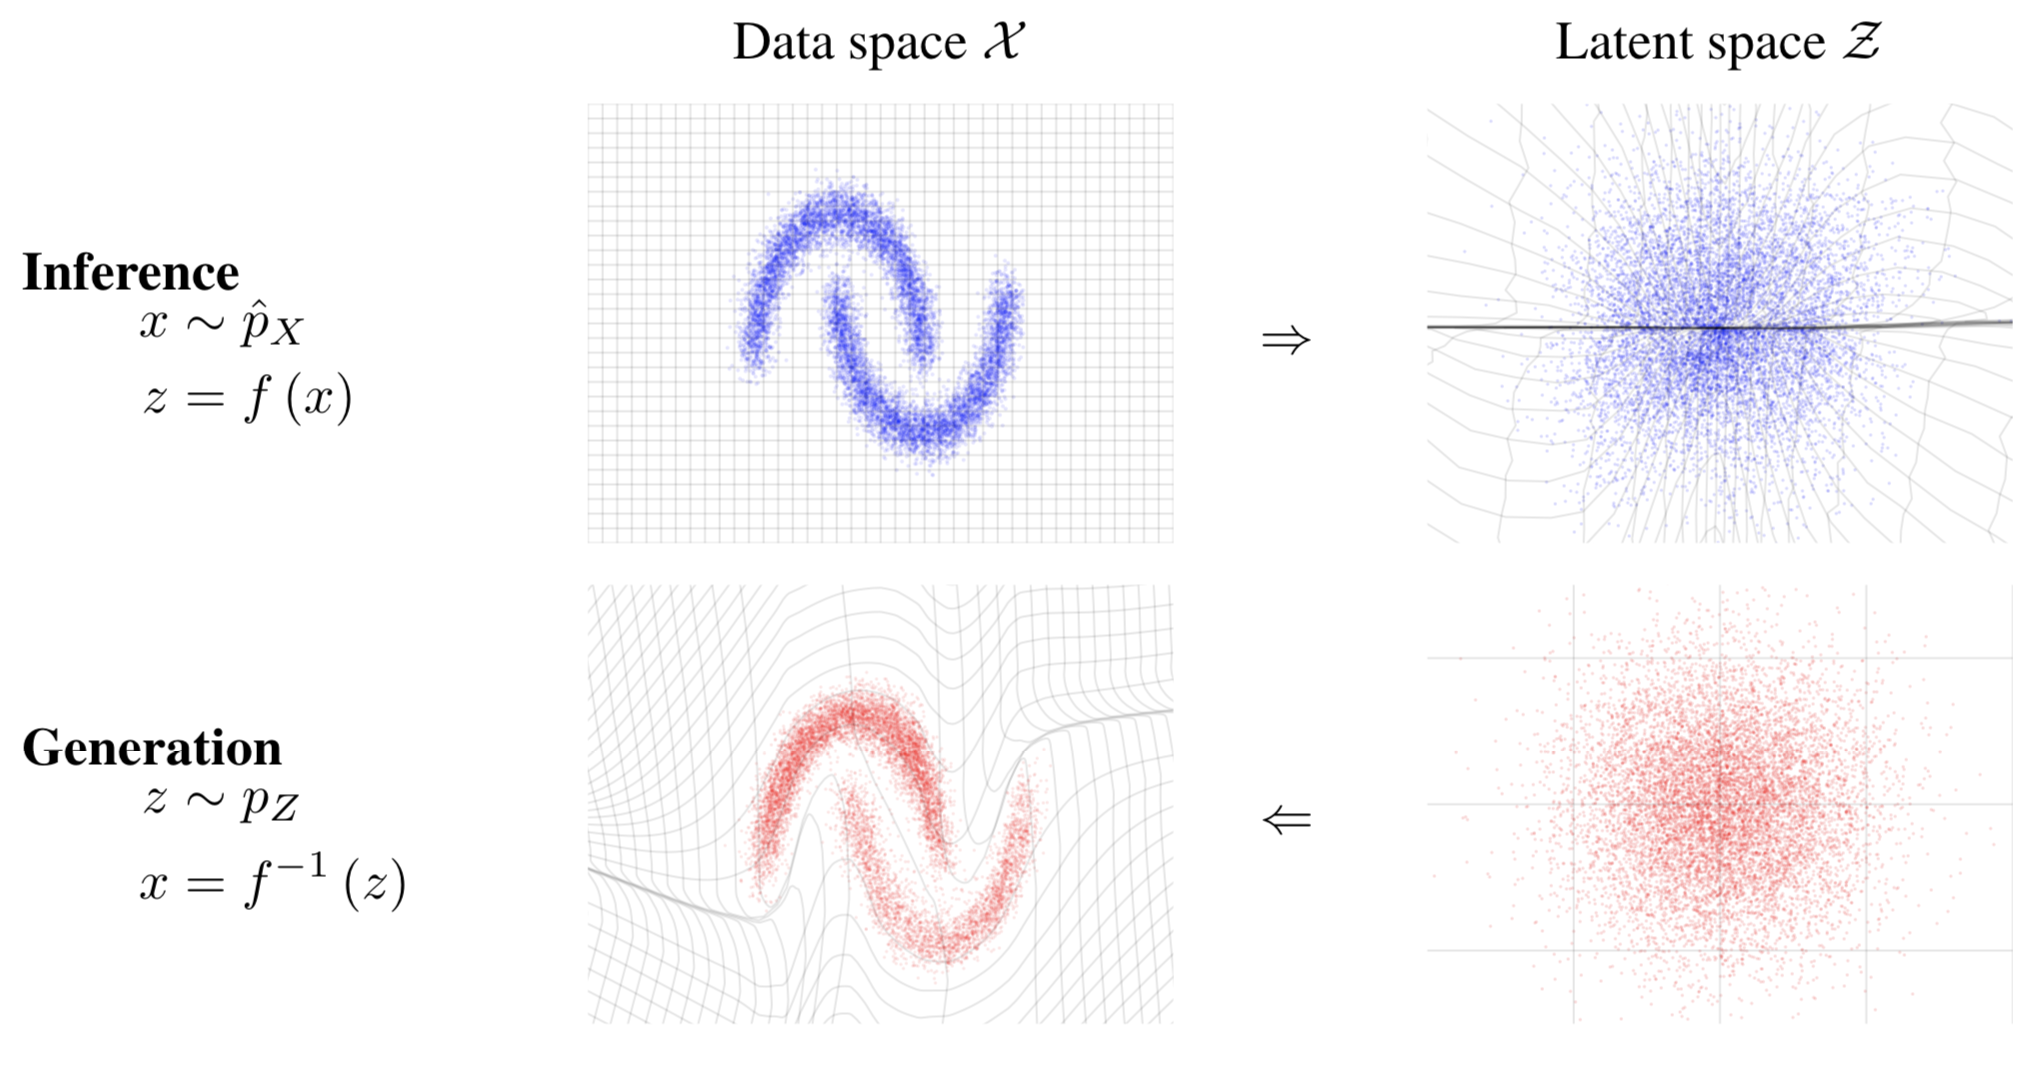
\includegraphics[width=0.85\linewidth]{figs/flows_how2}
	\end{figure}
	\myfootnotewithlink{https://arxiv.org/abs/1912.02762}{Papamakarios G. et al. Normalizing flows for probabilistic modeling and inference, 2019} 
\end{frame}
%=======
\begin{frame}{Normalizing flows KL duality}
	\begin{block}{Theorem}
		\vspace{-0.3cm}
		\[
			\argmin_{\btheta} KL(\pi(\bx) || p(\bx | \btheta)) = \argmin_{\btheta} KL(p(\bz | \btheta) || p(\bz)).
		\]
		\vspace{-0.5cm}
	\end{block}
	\begin{block}{Proof}
		\begin{itemize}
			\item $\bz \sim p(\bz)$, $\bx = \bg_{\btheta}(\bz)$, $\bx \sim p(\bx| \btheta)$;
			\item $\bx \sim \pi(\bx)$, $\bz = \bff_{\btheta}(\bx)$, $\bz \sim p(\bz | \btheta)$;
		\end{itemize}
		\vspace{-0.3cm}
		\begin{align*}
			\log p(\bz | \btheta) &= \log \pi(\bg_{\btheta}(\bz)) + \log | \det ( \bJ_\bg) |; \\
			\log p(\bx | \btheta) &= \log p(\bff_{\btheta}(\bx)) + \log | \det ( \bJ_\bff) |.
		\end{align*}
		\vspace{-0.9cm}
		\begin{multline*}
			KL\left(p(\bz | \btheta) || p(\bz) \right) = \mathbb{E}_{p(\bz | \btheta)} \bigl[ {\color{violet}\log p(\bz | \btheta)} - \log p(\bz) \bigr] = \\ 
			= \mathbb{E}_{{\color{olive}p(\bz | \btheta)}} \left[ {\color{violet}\log \pi(\bg_{\btheta}(\bz)) +  \log |\det (\bJ_\bg)|} - \log p(\bz) \right] = \\
			= \mathbb{E}_{{\color{olive}\pi(\bx)}} \left[ \log \pi(\bx) {\color{teal} - \log |\det (\bJ_\bff)| - \log p(\bff_{\btheta}(\bx))} \right] = \\
			= \mathbb{E}_{\pi(\bx)} \bigl[ \log \pi(\bx) {\color{teal} -\log p(\bx | \btheta)} \bigr] = KL (\pi(\bx) || p(\bx | \btheta)).
		\end{multline*}
	\end{block}
	\myfootnotewithlink{https://arxiv.org/abs/1705.07057}{Papamakarios G., Pavlakou T., Murray I. Masked Autoregressive Flow for Density Estimation, 2017} 
\end{frame}
%=======
\begin{frame}{Summary}
	\begin{itemize}
     	\item PixelCNN model use masked causal convolutions (1D or 2D) to get autoregressive model.
     	\vfill
		\item Change of variable theorem allows to get the density function of the random variable under the invertible transformation.
		\vfill
		\item Normalizing flows transform a simple base distribution to a complex one via a sequence of invertible transformations with tractable Jacobian.
		\vfill
		\item Normalizing flows have a tractable likelihood that is given by the change of variable theorem.
		\vfill
		\item We fit normalizing flows using forward or reverse KL minimization. 
	\end{itemize}
\end{frame}
\end{document} 